\usepackage{tikz}
\usetikzlibrary{arrows.meta, positioning, shapes.geometric, calc}

\section{Introduction}

Commercial organizations increasingly deploy large language model (LLM) agents into customer-facing and analytics-facing workflows: interactive dashboards that summarize marketing segments, tools that recommend next-best-actions, and chat-style assistants that call internal APIs to fetch data or trigger automations.
In these settings, an agent is not just ``a model'' but a \emph{service} governed by explicit contracts and expectations.
The service must emit JSON or other structured outputs that downstream systems can parse, must reflect the underlying data faithfully (e.g., segment statistics vs.\ population), and must respond within a reasonable time budget for an acceptable user experience.
If an agent claims that ``segment A has a higher conversion rate than the population'' when the opposite is true, or if the JSON response lacks required fields, it can lead to incorrect marketing decisions, broken dashboards, or even regulatory exposure.
If the agent is occasionally fast but frequently stalls at the tail, users perceive the whole system as unreliable.

Systems research has long emphasized that users experience \emph{tail latency}, not averages.
Dean and Barroso's ``The Tail at Scale'' \citep{dean2013tail} demonstrated that even a small fraction of slow requests can dominate perceived quality and limit throughput in large-scale services (see \url{https://cacm.acm.org/research/the-tail-at-scale/}).
Modern LLM-serving work extends this insight to Transformer inference.
Runtimes such as vLLM \citep{kwon2023vllm} (\url{https://arxiv.org/abs/2309.06180}), SGLang \citep{zheng2023sglang} (\url{https://arxiv.org/abs/2312.07104}), DeepSpeed-FastGen \citep{deepspeedFastGen} (\url{https://arxiv.org/abs/2401.08671}), and Sarathi-Serve \citep{agrawal2024sarathi} (\url{https://www.usenix.org/system/files/osdi24-agrawal.pdf}) propose kernel and scheduling optimizations---paged KV caches, optimized attention \citep{dao2023flashattention2,prabhu2024vattention}, speculative decoding \citep{leviathan2023speculative} (\url{https://arxiv.org/abs/2211.17192})---that improve throughput and reduce tail latency.
Yet these works largely treat the model as a black box that outputs free-form text, without explicit consideration of structured contracts or the \emph{semantic} correctness of responses.

In parallel, API providers and local runtimes have introduced \emph{structured output} modes.
OpenAI's structured outputs and function calling APIs (\url{https://openai.com/index/introducing-structured-outputs-in-the-api/}), Azure OpenAI, and Snowflake Cortex (\url{https://docs.snowflake.com/en/user-guide/snowflake-cortex/complete-structured-outputs}) expose JSON Schema-like contracts that models are expected to obey.
Local stacks such as LM Studio (\url{https://lmstudio.ai/docs/developer/openai-compat/tools}) and Ollama (\url{https://blog.danielclayton.co.uk/posts/ollama-structured-outputs/}) provide OpenAI-compatible endpoints with structured-output options.
Libraries like Outlines (\url{https://dottxt-ai.github.io/outlines/}), Instructor (\url{https://python.useinstructor.com/integrations/llama-cpp-python/}), and llama.cpp grammars (\url{https://github.com/ggml-org/llama.cpp/blob/master/grammars/README.md}) allow contracts to be compiled into regular languages or JSON constraints.
Recent benchmarks such as JSONSchemaBench and analyses of format constraints \citep{geng2025jsonschemabench,letmespeakfreely,structuredRAG} (\url{https://arxiv.org/abs/2501.10868}, \url{https://arxiv.org/abs/2408.02442}, \url{https://arxiv.org/abs/2408.11061}) show that constrained decoding substantially improves syntactic validity, but they leave open questions about interaction with serving runtimes, tail latency, and business-level metrics.

Beyond latency and shape, \emph{faithfulness}---whether an agent's textual summary is supported by the underlying data or retrieved context---has emerged as a central concern.
For a commercial analytics assistant that compares a segment's click-through rate (CTR), conversion rate, and churn markers to the population, it is not enough to produce grammatically correct prose; the summary must accurately reflect the statistics.
RAGAS (Retrieval Augmented Generation Assessment) \citep{es2023ragas} (\url{https://arxiv.org/abs/2309.15217}) proposed a set of automated metrics for retrieval-augmented generation (RAG) by using a judge model to score faithfulness and answer relevance.
Other work on ``atomic fact'' evaluation \citep{atomicFacts2024} (\url{https://arxiv.org/abs/2408.15171}) advocates decomposing responses into fine-grained statements and checking each against the context, to better understand hallucinations and subtle mistruths.
However, these frameworks are mostly experimental and are not yet tied tightly to production SLOs or to structured outputs that feed dashboards and scoring systems.

At the same time, cloud providers and tooling ecosystems have begun to articulate agent evaluation methods for production use.
Google's Agent Development Kit (ADK) and Vertex AI Generative AI evaluation documentation (\url{https://google.github.io/adk-docs/evaluate/}, \url{https://cloud.google.com/vertex-ai/generative-ai/docs/models/evaluation-overview}) advocate evaluating both \emph{final response quality} and \emph{trajectory quality} (tools invoked, step counts, error handling) using golden sets and metrics that matter to the business.
Google Cloud's blogs on agent testing and evaluation (\url{https://medium.com/google-cloud/agent-testing-and-evaluation-methods-64d1bd9ac44f}, \url{https://cloud.google.com/blog/topics/developers-practitioners/a-methodical-approach-to-agent-evaluation/}) and the LLM-Evalkit tools (\url{https://github.com/GoogleCloudPlatform/generative-ai/tree/main/tools/llmevalkit}, \url{https://cloud.google.com/blog/products/ai-machine-learning/introducing-llm-evalkit}) offer practical recipes for building evaluation pipelines.
However, these resources are high-level and platform-specific; they do not define a \emph{concrete, portable test suite} that ties together structured outputs, faithfulness metrics, trajectory checks, and SLO curves for agents running on local backends like LM Studio, Ollama, or vLLM.

In this work, we focus on the regime where a commercial team runs a \emph{single-GPU} agent stack---for example, an RTX 4090 in a small on-premise box or a MacBook Pro with Apple Silicon---and serves an analytics or CX agent via local OpenAI-compatible servers (e.g., LM Studio: \url{https://lmstudio.ai/docs/developer/openai-compat/tools}; Ollama: \url{https://docs.ollama.com/capabilities/structured-outputs}).
The agent must generate JSON reports and summaries that are both structurally correct and faithful to internal data (e.g., segment vs population stats), while respecting p95/p99 latency budgets and not over-consuming compute.
Practically, this scenario is common: teams want to avoid sending sensitive data to external APIs, want predictable costs, and still want high-quality agent behavior.
Crucially, in many of these use cases, \emph{correctness and truthfulness are prioritized over speed}, except where a specific real-time SLA explicitly dominates.

We argue that what is missing is a \textbf{spec-driven, SLO-aware evaluation and serving framework} that:
(i) treats JSON Schemas and grammars as the primary interface between application and LLM;
(ii) assesses not only syntactic validity but also content accuracy and faithfulness at the statement level;
(iii) measures and enforces tail-latency SLOs (p50/p95/p99, Success@\slo); and
(iv) is designed to run on single-GPU local backends rather than assuming massive serving clusters.
Such a framework should support both \emph{static evaluation} of a given policy and model, and \emph{dynamic evaluation} within a reinforcement learning loop, so that agents can improve and correct their behavior over time.

We contribute three main elements toward this goal.
First, we introduce a \emph{spec-to-decoder compilation layer} that translates JSON Schemas and grammars into constraints for LM Studio, Ollama, vLLM, and llama.cpp, with bounded validation-and-retry logic to preserve both contract adherence and latency.
Second, we design an \emph{auditable agent evaluation framework} built around a 100+ test suite that covers structural correctness, task accuracy, faithfulness (via an LLM judge adapted from RAGAS-style evaluation), tool-call and trajectory behavior, stability across seeds, and SLO adherence; this framework is configured via a canonical YAML file and produces detailed Weights \& Biases (W\&B) and Weave logs for reproducibility (\url{https://docs.wandb.ai/models/quickstart}, \url{https://docs.wandb.ai/models/artifacts}, \url{https://docs.wandb.ai/models/evaluate-models}).
Third, we describe how these metrics can be mapped to scalar rewards and constraints in a single-GPU reinforcement learning loop (e.g., TRL PPO/GRPO with LoRA adapters \citep{schulman2017ppo,grpo,dettmers2023qlora}, see \url{https://huggingface.co/docs/trl/en/logging} and \url{https://huggingface.co/docs/trl/en/grpo_trainer}), enabling agents to become more accurate and reliable over time while remaining within latency budgets.

The remainder of this paper is organized as follows.
Section~\ref{sec:background} reviews systems work on LLM serving and structured decoding, and agent evaluation frameworks from the cloud ecosystem.
Section~\ref{sec:problem} formulates spec-driven serving with SLOs as a constrained optimization problem.
Section~\ref{sec:method} describes our spec-to-decoder compilation, budgeted self-consistency, and SLO-aware serving methods.
Section~\ref{sec:eval-framework} presents the evaluation framework and the 100+ test suite in detail, including our faithfulness scorer and trajectory tests.
Section~\ref{sec:experiments} reports preliminary single-GPU experiments and ablations for structured decoding overhead and scheduling policies.
Section~\ref{sec:discussion} discusses limitations and future directions, including safety, multi-turn conversations, and more advanced RL integration.
\end{document}

\section{Background and Related Work}
\label{sec:background}

Our work sits at the intersection of systems for LLM serving, structured decoding and program synthesis, automated evaluation of language model outputs (especially faithfulness), and emerging agent evaluation frameworks used in production environments.
This section reviews prior work in each of these areas and highlights the gaps our spec-driven, SLO-aware framework seeks to fill.

\subsection{Tail Latency and LLM Serving on Commodity Hardware}

Traditional systems research has emphasized that users experience the worst-case behavior of a service rather than average latency.
Dean and Barroso's seminal article ``The Tail at Scale''~\citep{dean2013tail} (\url{https://cacm.acm.org/research/the-tail-at-scale/}) demonstrates that even a small fraction of slow requests can dominate overall user experience and limit system scalability.
They argue for design principles that explicitly target tail latency (e.g., \pninetyfive, \pninetynine) and highlight the need for multi-replica hedging, redundancy, and careful resource management.

LLM-serving work inherits these concerns and further complicates them due to high per-request compute costs and long, variable-length outputs.
vLLM introduces PagedAttention to provide efficient KV-cache management and continuous batching, significantly improving throughput for transformer models~\citep{kwon2023vllm} (\url{https://arxiv.org/abs/2309.06180}).
SGLang focuses on efficient execution of structured language model programs and proposes system-level optimizations (e.g., speculative execution of subprograms)~\citep{zheng2023sglang} (\url{https://arxiv.org/abs/2312.07104}).
DeepSpeed-FastGen~\citep{deepspeedFastGen} (\url{https://arxiv.org/abs/2401.08671}) and vAttention~\citep{prabhu2024vattention} (\url{https://arxiv.org/abs/2405.04437}) propose kernel- and memory-layout optimizations that reduce compute and memory overhead, further helping tail latency.
FlashAttention-2~\citep{dao2023flashattention2} (\url{https://arxiv.org/abs/2307.08691}) redesigns the attention kernel for better parallelism and cache usage.
Speculative decoding, as described by Leviathan \etal~\citep{leviathan2023speculative} (\url{https://arxiv.org/abs/2211.17192}), drafts tokens with a smaller model and verifies them with the target model to reduce time-to-first-token.

Sarathi-Serve~\citep{agrawal2024sarathi} (\url{https://www.usenix.org/system/files/osdi24-agrawal.pdf}) takes a more holistic view of throughput-latency trade-offs for LLM inference, examining queueing models and scheduling policies under realistic traffic patterns.
However, these works primarily consider text generation in isolation and often assume multi-GPU clusters; they do not directly address small-team, single-GPU setups where the same machine runs both the serving stack and other business workloads.
Furthermore, they typically ignore the semantics of outputs (e.g., JSON validity, schema adherence) and treat all text as equally valid as long as the model produces it fast enough.

In contrast, our focus is on single-GPU serving (RTX 4090 or equivalent, Apple M-series) for commercial analytics agents, where \emph{correctness and faithfulness} of the output are prioritized over pure speed except where latency is explicitly paramount.
We build on the scheduling and kernel-level insights from vLLM, Sarathi-Serve, DeepSpeed-FastGen, and FlashAttention-2, but we integrate these with contract-first decoding (Section~\ref{sec:method}) and a multi-metric evaluation suite tailored to structured agent use cases.

\subsection{Structured Outputs, Grammars, and Contract-First Decoding}

Real-world applications rarely want free-form text; they want structured outputs: JSON documents, typed objects, or tool-call payloads.
API providers have responded with structured-output modes.
OpenAI introduced function calling and structured outputs (see the blog post at \url{https://openai.com/index/introducing-structured-outputs-in-the-api/}), which allow developers to specify a JSON Schema-like specification that the model must adhere to.
Azure OpenAI and Snowflake Cortex offer similar capabilities for structured completions (\url{https://docs.snowflake.com/en/user-guide/snowflake-cortex/complete-structured-outputs}).

Local runtimes mirror these trends.
LM Studio provides an OpenAI-compatible developer interface for local models, including function calling and structured outputs (\url{https://lmstudio.ai/docs/developer/openai-compat/tools}).
Ollama has documented structured outputs via JSON-mode completions and blog posts about why structured outputs are critical (\url{https://blog.danielclayton.co.uk/posts/ollama-structured-outputs/}).
Fireworks.ai advocates for structured output modes across all LLMs, emphasizing error reduction and easier integration with application code (\url{https://fireworks.ai/blog/why-do-all-LLMs-need-structured-output-modes}).

Beyond provider-specific features, open-source libraries and runtimes provide generic contract-first tooling.
Outlines (\url{https://dottxt-ai.github.io/outlines/}) implements a grammar-based decoding layer that can enforce regular languages, JSON grammars, and Pydantic models on top of arbitrary providers.
`llama.cpp` supports grammars via GBNF (\url{https://github.com/ggml-org/llama.cpp/blob/master/grammars/README.md}), enabling constrained decoding even with local C++ inference.
Instructor (\url{https://python.useinstructor.com/integrations/llama-cpp-python/}) layers structured decoding on `llama-cpp-python` with validation and type-checked object construction.

Recent benchmark efforts specifically investigate structured generation.
JSONSchemaBench and related work \citep{geng2025jsonschemabench} (\url{https://arxiv.org/abs/2501.10868}) propose standardized JSON Schema tasks to test the ability of LLMs to follow structured contracts.
Studies of format constraints \citep{letmespeakfreely,structuredRAG} (\url{https://arxiv.org/abs/2408.02442}, \url{https://arxiv.org/abs/2408.11061}) show that forced formatting can influence model behavior and may trade off with other qualities (e.g., verbosity, creativity).
However, these works primarily measure static adherence to schemas or text-format constraints in isolation; they generally do not analyze the interaction between structured decoding and serving runtimes or between structured decoding and multi-dimensional evaluation metrics in a commercial agent context.

Our work is complementary: we treat structured decoding as one layer in a larger agent stack.
We show how to compile JSON Schemas and grammars into different serving backends (LM Studio, vLLM, llama.cpp) and evaluate not just schema adherence but also faithfulness, tool correctness, trajectory quality, and SLO adherence.
In particular, we target agents that generate JSON-based reports and summaries for analytics dashboards, where violating a schema or misrepresenting business metrics directly affects end users.

\subsection{Automated Evaluation of Faithfulness and Factuality}

Evaluating the truthfulness or faithfulness of LLM outputs is challenging, especially when ground truth is complex or partially implicit.
RAGAS (Retrieval Augmented Generation Assessment)~\citep{es2023ragas} (\url{https://arxiv.org/abs/2309.15217}) proposes a set of automatic metrics for RAG systems, including \emph{faithfulness} (does the answer contradict the context?) and \emph{answer correctness}.
RAGAS typically uses an LLM-as-judge: a judge model receives the context and answer and outputs a score.
This design has inspired many RAG evaluation pipelines in industry and open-source tools.

Other work advocates for decomposing responses into ``atomic facts'' and scoring the factuality of each, which improves interpretability and reduces the risk that a single aggregate score hides critical errors.
Kriman \etal~\citep{atomicFacts2024} (\url{https://arxiv.org/abs/2408.15171}) propose such atomic-fact–based evaluation for summarization.
Our commercial use case of segment vs population summaries is highly compatible with this paradigm: a short narrative can be decomposedinto statements like ``Segment A has higher CTR than the population'' or ``Segment B skews younger than the population'', each of which can be checked against numerical statistics.

However, recent work also points out that LLM-as-judge setups can be biased and unstable.
For example, studies ask questions such as "Are Large Language Models Fair Evaluators?" (e.g.,~\url{https://arxiv.org/abs/2305.17926}) and show that LLM judges can exhibit positional bias, oversensitivity to phrasing, or preferences for more verbose answers.
This raises concerns about using LLMs as sole judges for high-stakes applications.

Our framework adopts the insights of RAGAS and atomic-fact evaluation but makes several pragmatic adaptations:
(i) we restrict the domain to structured, numeric segment/population summaries where the context is precise;
(ii) we use a 0--3 support scale with an explicit contradiction flag, which increases the granularity of feedback;
(iii) we calibrate the judge using a small human-labeled set; and
(iv) we treat the judge as one signal among many, not the sole arbiter of agent quality.
These design choices align better with commercial analytics scenarios where numeric correctness is paramount and where evaluation noise must be minimized.

\subsection{Agent Evaluation Frameworks in Practice}

Cloud providers and tool vendors have begun to systematize agent evaluation.
Google's Agent Development Kit (ADK) documentation on ``Why Evaluate Agents'' (\url{https://google.github.io/adk-docs/evaluate/}) argues that agents should be tested both on final response quality and on the quality of trajectories (choices of tools, sequences, error handling).
Google Cloud's blog post ``Agent testing and evaluation methods'' (\url{https://medium.com/google-cloud/agent-testing-and-evaluation-methods-64d1bd9ac44f}) and the follow-up ``A methodical approach to agent evaluation'' (\url{https://cloud.google.com/blog/topics/developers-practitioners/a-methodical-approach-to-agent-evaluation/}) provide high-level recommendations: build golden test sets, define task-specific scoring rubrics, measure coverage, and use evaluation to gate deployments.
Vertex AI's evaluation overview (\url{https://cloud.google.com/vertex-ai/generative-ai/docs/models/evaluation-overview}) and the LLM-Evalkit tools (\url{https://github.com/GoogleCloudPlatform/generative-ai/tree/main/tools/llmevalkit}, \url{https://cloud.google.com/blog/products/ai-machine-learning/introducing-llm-evalkit}) offer concrete patterns and code samples for building evaluation pipelines around Vertex-hosted agents.

These resources are valuable as practical guides and establish a vocabulary for agent evaluation (e.g., golden sets, unit tests for agents, human-in-the-loop scoring).
However, they are tied to specific cloud environments and often assume that the serving runtime, model, and evaluation tooling live on the same platform.
They also typically focus on final response quality and loosely defined ``agent success'' rather than enumerating detailed tests for structure, faithfulness, tool behavior, stability, and SLOs that can be ported to local, single-GPU setups.

Our work generalizes these practices by:
(i) defining a portable, backend-agnostic test suite (100+ tests) that can run on LM Studio, Ollama, vLLM, or cloud APIs;
(ii) expressing the suite in a declarative YAML format so it can be consumed by different evaluation runners (e.g., LLM-Evalkit, custom harnesses, Weave workflows); and
(iii) integrating evaluation results with RL training loops and CI pipelines using W\&B online logging (\url{https://docs.wandb.ai/models/quickstart}, \url{https://docs.wandb.ai/models/artifacts}, \url{https://docs.wandb.ai/models/evaluate-models}, \url{https://huggingface.co/docs/trl/v0.14.0/en/logging}).

\subsection{Single-GPU Local Serving and Open-Weight Models}

A key difference between many academic systems papers and our target setting is the hardware and deployment model.
Instead of assuming large clusters or managed APIs, we assume that the agent runs on \emph{commodity hardware} (e.g., a single RTX 4090) or a developer laptop (e.g., MacBook Pro with Apple M2 Max), using local servers such as LM Studio or Ollama.

LM Studio documentation describes how to run a local OpenAI-compatible endpoint (\url{https://lmstudio.ai/docs/developer/openai-compat/tools}) and how to load open-weight models like Qwen3 (\url{https://lmstudio.ai/models}).
Qwen's documentation provides instructions for running models locally and via OpenAI-compatible APIs (\url{https://qwen.readthedocs.io/en/latest/getting_started/quickstart.html}).
Ollama offers a simple command-line and API interface to run models locally with optional structured outputs (\url{https://docs.ollama.com/capabilities/structured-outputs}).
These tools make it possible for small teams to serve LLM agents without sending data to external vendors, but they do not prescribe a particular evaluation methodology or SLO policy.

Open-source projects such as vLLM (often used with Qwen via recipes like \url{https://modal.com/docs/examples/vllm_inference}) and llama.cpp provide high-performance serving for open-weight models.
Our framework is designed to sit above these runtimes: it does not depend on any specific vendor but assumes an OpenAI-compatible API and the ability to log rich metadata (latency, token counts, prompts, responses) to W\&B for analysis.

By focusing explicitly on single-GPU local serving for a commercial analytics assistant, we bridge the gap between large-scale, research-oriented serving work and the needs of teams that want to deploy agents realistically in their own infrastructure.
Our background review motivates the need for a unifying approach that brings together structured decoding, faithfulness evaluation, agent trajectory analysis, SLO tracking, and RL optimization.
The next section formalizes this problem setting and introduces the spec-driven, SLO-aware agent serving objective we consider.

\section{Problem Formulation}
\label{sec:problem}

Figure~\ref{fig:agent-context} sketches the setting we target.
A generic commercial agent sits between upstream requesters (users, other systems) and downstream consumers (dashboards, workflows, humans).
The agent reads unstructured and structured context (documents, logs, records, prior turns), optionally calls tools (APIs, databases, services), and is expected to emit structured outputs such as JSON reports, action recommendations, or tool-call payloads.
These outputs flow not only to a chat UI, but also into critical systems such as campaign engines, scoring pipelines, or compliance dashboards.
In such environments, small model errors can propagate and compound: a malformed JSON object may crash a downstream job; a misleading summary may cause a manager to launch the wrong campaign; a subtle numerical hallucination may misreport risk.
At the same time, users expect the agent to be responsive: if a dashboard feels “hung,” trust erodes even if the answers are technically correct.

Our goal is to make this setting precise in a way that is \emph{both} amenable to systems-level analysis (latency, throughput, SLOs) and \emph{fine-grained} enough to capture semantics (structure, task accuracy, faithfulness, tool behavior, stability).
We do this by defining: (i) a general agent and contract model, (ii) a serving environment with latency-based SLOs, and (iii) a vector of evaluation metrics and a configuration file that converts them into pass/fail gates and scalar scores.
Figure~\ref{fig:metric-families} provides a visual taxonomy of the metric families we use; Figure~\ref{fig:optimization-view} provides an optimization view that will motivate static selection and RL-based policy improvement.

\subsection{Agent and Contract Model}

An \emph{agent invocation} corresponds to a single request--response episode.
Let $\mathcal{X}$ denote the space of requests.
Each $x \in \mathcal{X}$ may consist of:
\begin{itemize}[leftmargin=12pt]
    \item a user instruction or task description (free-form text or a structured spec),
    \item a set of context items $C = \{c_1,\dots,c_m\}$ such as retrieved documents, knowledge base entries, prior conversation turns, or database records,
    \item optional metadata such as user profile, locale, or authorization context.
\end{itemize}
We do not constrain the domain: $x$ might encode an analytics query, a support ticket, an internal “runbook” request, or a code-editing task.

For each request $x$, the agent must produce one or more outputs $y$ in an output space $\mathcal{Y}$; $\mathcal{Y}$ is defined by a \emph{contract} $\mathcal{C}$.
In practical systems, contracts are expressed as JSON Schemas, Pydantic models, protocol buffer definitions, or even context-free grammars.
We abstract this as a predicate
\[
\mathcal{C} : \mathcal{Y} \to \{0,1\}
\]
that returns $1$ if and only if $y$ is syntactically well-formed (e.g., valid JSON) and satisfies all structural constraints (field presence, types, enum values, bounds, nesting) and any additional schema invariants.
When we say “contract-first,” we mean that $\mathcal{C}$ is defined \emph{before} the agent is invoked and that the decoding process is explicitly designed to obey it.

We consider a parametric policy $\pi_\theta$, typically an LLM with prompts and, optionally, fine-tuned weights.
The policy is deployed via a serving runtime $R$ (e.g., LM Studio, Ollama, vLLM, or llama.cpp) that exposes an OpenAI-compatible API.
Given a request $x$, contract $\mathcal{C}$, and decoding configuration $\delta$ (temperature, top-$p$, maximum tokens, number of samples $k$ for self-consistency, etc.), the agent induces a distribution over outputs:
\[
y \sim \pi_\theta(\cdot \mid x, \mathcal{C}, \delta, R).
\]
Because $R$ may support structured-output features (e.g., OpenAI-style \texttt{response\_format}, see \url{https://openai.com/index/introducing-structured-outputs-in-the-api/}, LM Studio docs at \url{https://lmstudio.ai/docs/developer/openai-compat/tools}, Ollama structured outputs at \url{https://docs.ollama.com/capabilities/structured-outputs}), we distinguish between:
\begin{itemize}[leftmargin=12pt]
    \item \emph{provider-native constraints}, where $\mathcal{C}$ is translated into a schema or grammar understood by the serving runtime, and
    \item \emph{library-based or post-hoc constraints}, where $\mathcal{C}$ is enforced via tools such as Outlines (\url{https://dottxt-ai.github.io/outlines/}) or llama.cpp grammars (\url{https://github.com/ggml-org/llama.cpp/blob/master/grammars/README.md}) and validation-and-retry logic.
\end{itemize}
From the agent’s perspective, the contract and the decoding configuration are part of the “policy”: if we change $\mathcal{C}$ or $\delta$, we effectively change the behavior of $\pi_\theta$.

\subsection{Serving Environment and Latency SLOs}

We assume the agent stack runs on a \emph{single, finite-capacity node} equipped with a GPU (e.g., RTX 4090) or a laptop-class accelerator (e.g., Apple M2 Max).
The serving runtime $R$ handles prefill and decoding, possibly batching multiple requests and managing KV caches as in vLLM (\url{https://arxiv.org/abs/2309.06180}) or similar systems.
For each request $x$, we measure the end-to-end latency
\[
L(x) = t_{\text{finish}}(x) - t_{\text{start}}(x),
\]
where the start time is when the request is submitted to $R$ and the finish time is when a fully validated structured output $y$ (or an error) is available to downstream consumers.

In a realistic environment, requests arrive according to a stochastic process that may include bursts, diurnal patterns, and varying context sizes.
Let $Q(R,\pi_\theta,\delta)$ denote the distribution of latencies induced by deploying $(R,\pi_\theta,\delta)$ under a workload model that approximates production traffic.
We characterize tail latency by quantiles such as $\mathrm{p50}(Q)$, $\mathrm{p95}(Q)$, and $\mathrm{p99}(Q)$.
Following \citet{dean2013tail}, we treat $\mathrm{p95}(Q)$ and $\mathrm{p99}(Q)$ as first-class metrics: they govern perceived responsiveness and throughput.

Commercial teams typically express latency-related requirements as service-level objectives (\slo s).
For example, a BI dashboard might demand that 95\% of agent responses complete within 1 second and 99\% within 2 seconds:
\[
\mathrm{p95}(Q) \leq B,\quad \mathrm{p99}(Q) \leq B',
\]
for budgets $B$ and $B'$ in milliseconds.
There may also be SLOs on time-to-first-token (TTFT), especially for chat-like UX.

Importantly, in many enterprise contexts, stakeholders place \emph{conditional priority} on metrics:
\begin{itemize}[leftmargin=12pt]
    \item First, the agent must be \emph{structurally and semantically correct}: JSON must parse and match schema, extracted fields must match ground truth or expected patterns, and summaries must be faithful to context.
    \item Second, given correctness, the agent should be stable across seeds and days; outputs should not fluctuate unpredictably.
    \item Third, given correctness and stability, latency should fall within agreed SLOs; exceptionally latency-critical applications are treated explicitly as such.
\end{itemize}
We encode this lexicographic preference in our evaluation criteria and reward design: latency is treated primarily as a constraint, not as the primary objective, except for use cases explicitly marked as speed-critical.

To capture the combined notion of “correct and fast enough,” we define an episode-level binary indicator:
\[
\text{Success@\slo}(x) =
\begin{cases}
1 & \text{if the episode satisfies both correctness/quality criteria and latency constraints},\\
0 & \text{otherwise.}
\end{cases}
\]
Correctness/quality is determined by metrics described next; latency constraints are determined by $B$ and $B'$.

\subsection{Metrics, Criteria, and Configuration via \texttt{criteria.yaml}}

To reason about agents in a way that is both auditable and tunable, we define a vector of metrics $m(x,y) \in \mathbb{R}^K$ for each episode.
Figure~\ref{fig:metric-families} summarizes the metric families; here we detail them and explain how they are configured.

\paragraph{Structural metrics.}
We compute:
\begin{itemize}[leftmargin=12pt]
    \item JSON parse success (1 if the model’s output can be parsed as JSON, 0 otherwise).
    \item Schema validity (1 if the JSON satisfies $\mathcal{C}$, 0 otherwise).
    \item Detailed error codes (missing required field, extra field, type mismatch, enum violation, size bounds), which are useful for debugging and RL shaping but may not contribute to a single scalar metric.
\end{itemize}

\paragraph{Task accuracy metrics.}
Where ground truth labels or references exist, we compute appropriate accuracy metrics:
\begin{itemize}[leftmargin=12pt]
    \item macro-F1 or micro-F1 on extracted fields;
    \item exact match for QA-style tasks;
    \item pass@1 or pass@k for code generation tasks.
\end{itemize}

\paragraph{Faithfulness metrics.}
We adopt a RAGAS-inspired faithfulness signal \citep{es2023ragas} and atomic-fact evaluation \citep{atomicFacts2024}.
Given a context $C$ (retrieved documents, internal data, etc.) and an output $y$, we use a judge model to:
(i) decompose $y$ into atomic statements;
(ii) assign each statement a support label $s \in \{0,1,2,3\}$ (from not supported to strongly supported);
(iii) flag contradictions between statements or with the context.
We then define a scalar $m_{\text{faith}}(x,y) \in [0,1]$ as a function of the fraction of strongly supported statements, the average support, and a penalty for contradictions.
The exact aggregation is configurable.

\paragraph{Tool and trajectory metrics.}
If the agent can call tools, we track:
\begin{itemize}[leftmargin=12pt]
    \item tool-call success (valid arguments, HTTP 2xx, no schema violations), $m_{\text{tool}}$;
    \item trajectory metrics: number of tool calls, invalid-argument retries, redundant calls, and edit distance to an expected tool sequence, inspired by Google’s ADK and Vertex agent evaluations (\url{https://google.github.io/adk-docs/evaluate/}, \url{https://cloud.google.com/vertex-ai/generative-ai/docs/models/evaluation-overview}).
\end{itemize}

\paragraph{Stability metrics.}
We measure stability via:
\begin{itemize}[leftmargin=12pt]
    \item Disagreement@$k$: for $k$ repeated runs with the same configuration (up to non-determinism in sampling), we compute 1 minus the fraction of runs that produce equivalent structured outputs or atomic-fact sets.
    \item Seed variance: variance of key metrics (F1, faithfulness) across runs with different random seeds, analogous to LLM stability analyses~\citep{llmStability} (\url{https://arxiv.org/abs/2408.04667}).
\end{itemize}

\paragraph{Latency and SLO metrics.}
For each episode, we record $L(x)$.
Over an evaluation set $\mathcal{D}_{\text{eval}}$, we compute p50, \pninetyfive, \pninetynine, as well as Success@\slo rates and other derived indicators (e.g., fraction of requests exceeding 2 seconds).

\medskip

All of these metrics, along with their thresholds and weights, are configured via \texttt{agent\_eval/criteria.yaml}.
This YAML file specifies:
\begin{enumerate}[leftmargin=12pt]
    \item which metrics are active (e.g., turning tool metrics on only when tools are used),
    \item pass/fail thresholds for each metric (e.g., JSON validity $\ge 0.99$, faithfulness $\ge 0.75$, Disagreement@$k \le 0.2$),
    \item weights for combining metrics into scalar scores for dashboards or reinforcement learning rewards.
\end{enumerate}
For example, it may define a composite score:
\[
\text{Score}(x,y) = w_{\text{task}} m_{\text{f1}} + w_{\text{faith}} m_{\text{faith}} + w_{\text{json}} m_{\text{json}} + w_{\text{tool}} m_{\text{tool}} + w_{\text{slo}} m_{\text{slo}} - \lambda_{\text{lat}} L(x) - \lambda_{\text{disc}} m_{\text{disc}},
\]
with $w_{\text{task}}, w_{\text{faith}}, w_{\text{json}}$ chosen large relative to $\lambda_{\text{lat}}$ to encode the preference for correctness and truthfulness over speed, except in explicitly latency-critical scenarios.

\subsection{Static Selection and Policy Improvement}

Figure~\ref{fig:optimization-view} provides an optimization view of the problem.
Given a configuration $(R,\pi_\theta,\delta)$, the agent interacts with requests from $\mathcal{X}$, the serving runtime produces outputs $y$, and the evaluation harness computes metrics $m(x,y)$.
Aggregating these metrics over an evaluation set yields performance summaries and scores that can be used for two purposes:

\begin{enumerate}[leftmargin=12pt]
    \item \textbf{Static selection.}
    Treat $(R,\pi_\theta,\delta)$ as a point in a configuration space.
    Use the evaluation framework to estimate aggregate performance $J(R,\pi_\theta,\delta)$ and check SLO-gated constraints.
    In this regime, one can perform grid search, Bayesian optimization, or bandit-style exploration over decoding and scheduling parameters with our composite score as the objective.
    This is analogous to what LLM-Evalkit provides for Vertex-hosted agents (\url{https://github.com/GoogleCloudPlatform/generative-ai/tree/main/tools/llmevalkit}), but our metric set is richer and supports local runtimes.
    \item \textbf{Policy improvement.}
    Interpret $\text{Score}(x,y)$ (or its components) as a reward signal in a Markov decision process (MDP) or constrained MDP.
    Using TRL's PPO or GRPO trainers (\url{https://huggingface.co/docs/trl/en/logging}, \url{https://huggingface.co/docs/trl/en/grpo_trainer}) with LoRA-based adapters~\citep{dettmers2023qlora}, we can iteratively update $\theta$ so that the agent improves over time on the dimensions defined in \texttt{criteria.yaml}, while keeping SLO-related costs bounded through Lagrangian or PID-style updates~\citep{achiam2017cpo,altman1999cmdp}.
\end{enumerate}

In both cases, the evaluation framework serves as the \emph{measurement} layer that powers both research (ablation studies, comparisons across backends) and practice (CI gates, rollout decisions, RL reward definitions).
In the rest of this paper we instantiate this problem formulation with concrete tasks and experiments and describe how spec-driven decoding and serving are implemented on single-GPU infrastructure.

\begin{figure}[t]
    \centering
    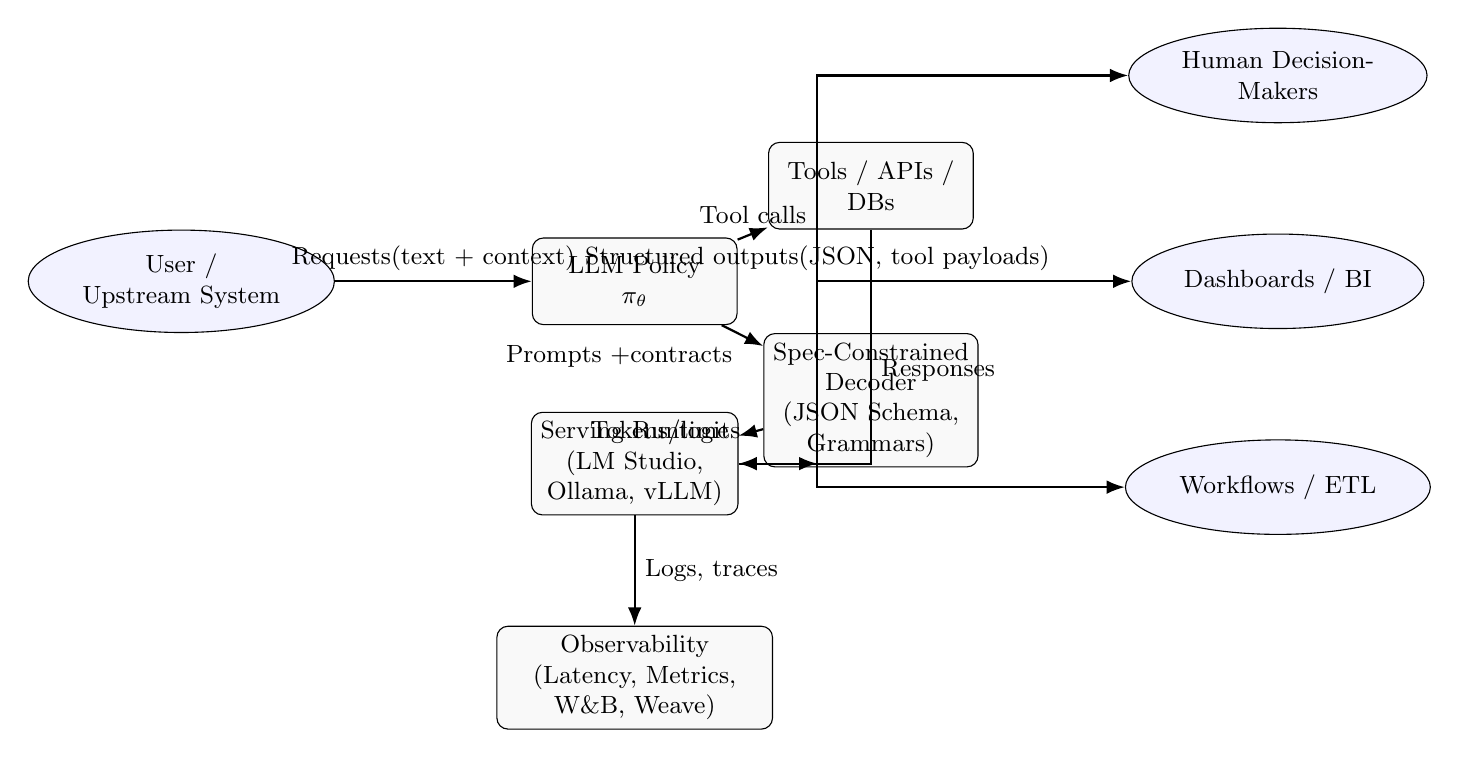
\begin{tikzpicture}[
        font=\small,
        node distance=1.8cm and 2.0cm,
        box/.style={draw, rounded corners, align=center, minimum width=2.6cm, minimum height=1.1cm, fill=gray!5},
        line/.style={-Latex, thick},
        cloud/.style={draw, ellipse, align=center, minimum width=2.5cm, minimum height=1.2cm, fill=blue!5}
    ]

    % Left: user / upstream
    \node[cloud] (user) {User /\\ Upstream System};

    % Middle: agent stack
    \node[box, right=2.5cm of user] (policy) {LLM Policy\\ $\pi_\theta$};
    \node[box, above=0.1cm of policy, xshift=3.0cm] (tools) {Tools / APIs /\\ DBs};
    \node[box, below=0.1cm of policy, xshift=3.0cm] (spec) {Spec-Constrained\\ Decoder\\ (JSON Schema,\\ Grammars)};
    \node[box, below=1.1cm of policy] (runtime) {Serving Runtime\\ (LM Studio,\\ Ollama, vLLM)};

    % Right: downstream
    \node[cloud, right=5.0cm of policy] (downstream1) {Dashboards / BI};
    \node[cloud, below=1.4cm of downstream1] (downstream2) {Workflows / ETL};
    \node[cloud, above=1.4cm of downstream1] (downstream3) {Human Decision-\\ Makers};

    % Arrows from user to policy
    \draw[line] (user) -- node[above]{Requests\\ (text + context)} (policy);

    % Policy to tools/decoder/runtime
    \draw[line] (policy) -- node[above]{Tool calls} (tools);
    \draw[line] (policy) -- node[below left]{Prompts +\\ contracts} (spec);
    \draw[line] (spec) -- node[left]{Tokens/\\ logits} (runtime);

    % Tools to runtime (responses)
    \draw[line] (tools) |- node[right,pos=0.3]{Responses} (runtime);

    % Runtime to downstream
    \draw[line] (runtime.east) -- ++(1.0,0) coordinate (midout);
    \draw[line] (midout) |- node[above]{Structured outputs\\ (JSON, tool payloads)} (downstream1.west);
    \draw[line] (midout) |- (downstream2.west);
    \draw[line] (midout) |- (downstream3.west);

    % Latency + logs
    \node[box, below=1.4cm of runtime, align=center, minimum width=3.5cm] (obs) {Observability\\ (Latency, Metrics,\\ W\&B, Weave)};
    \draw[line] (runtime.south) -- node[right]{Logs, traces} (obs.north);

    \end{tikzpicture}
    \caption{System context for a generic commercial agent. Requests flow from users or upstream systems into the agent stack, which consists of an LLM policy, tools/APIs, a spec-constrained decoder, and a serving runtime. Structured outputs (JSON, tool payloads) are consumed by dashboards, workflows, and humans. Latency and evaluation metrics are logged for analysis and RL-based improvement.}
    \label{fig:agent-context}
\end{figure}

\begin{figure}[t]
    \centering
    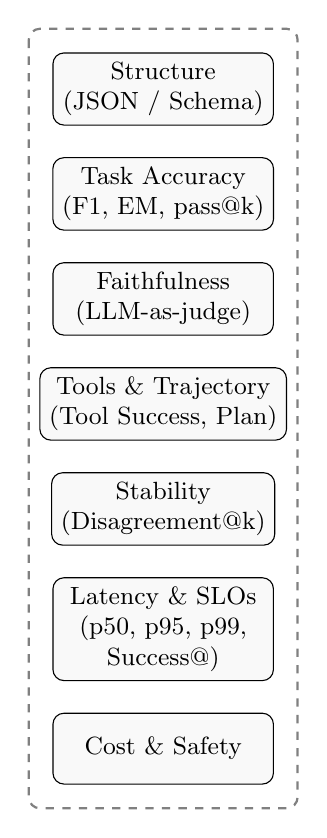
\begin{tikzpicture}[
        font=\small,
        category/.style={draw, rounded corners, minimum width=2.8cm, minimum height=0.9cm, align=center, fill=gray!5},
        node distance=0.4cm
    ]

    \node[category] (structure) {Structure\\ (JSON / Schema)};
    \node[category, below=of structure] (accuracy) {Task Accuracy\\ (F1, EM, pass@k)};
    \node[category, below=of accuracy] (faith) {Faithfulness\\ (LLM-as-judge)};
    \node[category, below=of faith] (tools) {Tools \& Trajectory\\ (Tool Success, Plan)};
    \node[category, below=of tools] (stability) {Stability\\ (Disagreement@k)};
    \node[category, below=of stability] (latency) {Latency \& SLOs\\ (p50, p95, p99,\\ Success@\slo)};
    \node[category, below=of latency] (cost) {Cost \& Safety};

    \draw[rounded corners, thick, dashed, gray] ($(structure.north west)+(-0.3,0.3)$) rectangle ($(cost.south east)+(0.3,-0.3)$);

    \end{tikzpicture}
    \caption{Metric families in our evaluation framework. We track structure (syntactic and schema validity), task accuracy, faithfulness to context, tool and trajectory behavior, stability across runs, latency/SLO metrics, and cost/safety. The concrete metrics and thresholds are configured centrally via \texttt{agent\_eval/criteria.yaml}.}
    \label{fig:metric-families}
\end{figure}

\begin{figure}[t]
    \centering
    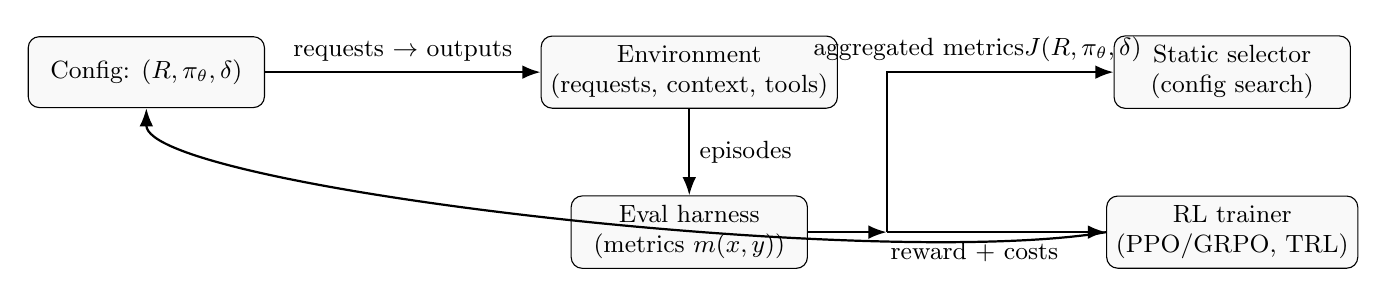
\begin{tikzpicture}[
        font=\small,
        node distance=1.8cm and 2.0cm,
        comp/.style={draw, rounded corners, minimum width=3.0cm, minimum height=0.9cm, align=center, fill=gray!5},
        line/.style={-Latex, thick}
    ]

    % Left: config
    \node[comp] (config) {Config: $(R,\pi_\theta,\delta)$};

    % Middle: environment + eval
    \node[comp, right=3.5cm of config] (env) {Environment\\ (requests, context, tools)};
    \node[comp, below=1.1cm of env] (eval) {Eval harness\\ (metrics $m(x,y)$)};

    % Right: selectors
    \node[comp, right=3.5cm of env] (selector) {Static selector\\ (config search)};
    \node[comp, below=1.1cm of selector] (rl) {RL trainer\\ (PPO/GRPO, TRL)};

    % Arrows
    \draw[line] (config) -- node[above]{requests $\to$ outputs} (env);
    \draw[line] (env) -- node[right]{episodes} (eval);

    \draw[line] (eval.east) -- ++(1.0,0) coordinate (mid);
    \draw[line] (mid) |- node[above,pos=0.7]{aggregated metrics\\ $J(R,\pi_\theta,\delta)$} (selector.west);
    \draw[line] (mid) |- node[below,pos=0.7]{reward + costs} (rl.west);

    % Feedback from RL to config
    \draw[line] (rl.west) .. controls +(-3, -0.5) and +(0,-1.0) .. (config.south);

    \end{tikzpicture}
    \caption{Optimization view. Given a configuration $(R,\pi_\theta,\delta)$, the environment and evaluation harness produce metrics $m(x,y)$ that are aggregated into performance summaries $J(R,\pi_\theta,\delta)$. These summaries drive static selection (config search) and policy improvement (SLO-aware RL using PPO/GRPO in TRL).}
    \label{fig:optimization-view}
\end{figure}

\section{Spec-Driven Decoding and Single-GPU Serving}
\label{sec:method}

Section~\ref{sec:problem} formalized our setting in terms of a policy $\pi_\theta$, a contract $\mathcal{C}$, a runtime $R$, a decoding configuration $\delta$, and evaluation metrics $m(x,y)$.
Figure~\ref{fig:agent-context} shows where these components live in the system: the contract and decoder sit between the LLM policy and the serving runtime, and their outputs feed downstream systems.
We now describe the design of this layer in detail: how contracts are represented, how they are compiled into provider-specific constraints, how we implement budgeted self-consistency and validation-and-retry, and how we tie these components to single-GPU runtime parameters and monitoring.

\subsection{Contract Representation and Internal Data Structures}
\label{sec:spec-representation-deep}

Our contract representation is built around JSON Schema, but we treat schemas as one view on top of an internal abstract syntax tree (AST).
This AST is designed to compile cleanly to JSON Schema for validation, to GBNF grammars for llama.cpp, and to provider-specific hints (e.g., OpenAI's \texttt{response\_format}).

\paragraph{JSON Schema view.}
We define a minimal internal type system:
\begin{itemize}[leftmargin=12pt]
    \item scalar types: \texttt{string}, \texttt{number}, \texttt{integer}, \texttt{boolean};
    \item composite types: \texttt{object}, \texttt{array};
    \item constraints: required fields, enum values, range constraints, length constraints, nested schemas.
\end{itemize}
The following example illustrates a simple contract for a generic agent response:
\begin{lstlisting}[language=json,basicstyle=\ttfamily\small]
{
  "type": "object",
  "properties": {
    "short_description": { "type": "string" },
    "details": {
      "type": "object",
      "properties": {
        "main_points": {
          "type": "array",
          "items": { "type": "string" },
          "minItems": 1, "maxItems": 10
        },
        "risk_score": {
          "type": "number",
          "minimum": 0.0, "maximum": 1.0
        }
      },
      "required": ["main_points"]
    }
  },
  "required": ["short_description", "details"],
  "additionalProperties": false
}
\end{lstlisting}
Internally, this is parsed into an AST with nodes for each property and constraints.
We store a canonical JSON Schema form (for validation and providers like OpenAI/LM Studio, see \url{https://openai.com/index/introducing-structured-outputs-in-the-api/} and \url{https://lmstudio.ai/docs/developer/openai-compat/tools}) and a richer structure for grammar compilation.

\paragraph{Grammar view.}
Certain backends (e.g., llama.cpp) accept grammars (GBNF) that constrain output sequences.
We map the AST to a grammar by:
\begin{enumerate}[leftmargin=12pt]
    \item emitting production rules for objects and arrays (e.g., \texttt{"\{" field ("," field)* "\}"} with appropriate field rules);
    \item encoding scalar types as appropriate character/token classes (e.g., JSON strings, numeric patterns);
    \item factoring enum constraints into choice productions.
\end{enumerate}
For example, \texttt{"short\_description"} becomes a rule that enforces a quoted string; \texttt{"risk\_score"} becomes a rule that matches a floating point in [0,1] (optionally enforced via post-hoc checks, since range constraints are awkward to express in grammars).
We reuse patterns from llama.cpp's grammar documentation (\url{https://github.com/ggml-org/llama.cpp/blob/master/grammars/README.md}).

\paragraph{Typed view.}
We optionally maintain a typed view (e.g., Pydantic model) that provides static typing for developer experience and runtime checks.
Tools like Instructor (\url{https://python.useinstructor.com/integrations/llama-cpp-python/}) use this view to automatically validate model outputs and construct Python objects.

\subsection{Spec Compiler: From Contracts to Decoding Configurations}
\label{sec:spec-compiler}

Given an internal contract AST, the \emph{spec compiler} builds per-backend artifacts:

\begin{itemize}[leftmargin=12pt]
    \item for OpenAI-compatible runtimes (OpenAI, Azure, LM Studio, Fireworks):
    \begin{itemize}[leftmargin=12pt]
        \item JSON Schema string for \texttt{response\_format} or function schemas;
        \item optional system prompt snippets reminding the model of the structure.
    \end{itemize}
    \item for grammar-based runtimes (Outlines, llama.cpp):
    \begin{itemize}[leftmargin=12pt]
        \item a GBNF grammar file that enforces basic structure;
        \item mapping between grammar rules and schema fields for downstream evaluation.
    \end{itemize}
    \item for validation and debugging:
    \begin{itemize}[leftmargin=12pt]
        \item a JSON Schema used with a validator (e.g., \texttt{jsonschema} in Python);
        \item a deterministic field ordering used when reconstructing or comparing outputs.
    \end{itemize}
\end{itemize}

At runtime, the compiler is invoked with a target backend identifier (e.g., \texttt{backend="lmstudio"} or \texttt{backend="llama\_cpp"}), and it returns a \emph{decoder configuration object} that includes:
\begin{itemize}[leftmargin=12pt]
    \item provider-specific parameters (e.g., \texttt{response\_format} payloads, grammar file paths);
    \item a validator handle for post-hoc checks;
    \item any necessary metadata for Weave/W\&B logging (e.g., schema version, grammar hash).
\end{itemize}

This design decouples application contracts from backend-specific details.
Changing from LM Studio to Ollama or vLLM requires changing backend flags and endpoints, not rewriting schema logic.

\subsection{Budgeted Self-Consistency: Algorithm and Complexity}
\label{sec:self-consistency-deep}

Self-consistency is a powerful tool for improving reliability but can be expensive if uncontrolled.
We therefore implement a \emph{budgeted} self-consistency procedure that respects wall-clock and token budgets.

Let $B_{\text{wall}}$ be the maximum allowed wall-clock time for generating alternative candidates, $C_{\text{tokens}}$ the maximum total number of tokens (sum of all candidates), and $k_{\max}$ the maximum number of samples.
We implement self-consistency as in Algorithm~\ref{alg:self-consistency}.

\begin{figure}[t]
\begin{lstlisting}[language=Python,basicstyle=\ttfamily\small,caption={Pseudocode for budgeted self-consistency with structured decoding.},label={alg:self-consistency}]
def budgeted_self_consistency(x, contract, runtime, policy, config,
                              wall_budget_ms, token_budget, k_max):
    start = now_ms()
    candidates = []
    total_tokens = 0

    for k in range(k_max):
        if now_ms() - start > wall_budget_ms:
            break
        if total_tokens >= token_budget:
            break

        # 1) structured decode with compiled contract
        y_k, info = structured_decode(
            x, contract, runtime, policy, config
        )
        total_tokens += info.tokens_generated

        # 2) validate against contract
        valid, errors = validate(y_k, contract)
        if not valid:
            # log error type, continue if budget allows
            log_validation_error(errors)
            continue

        # 3) optional faithfulness scoring with judge model
        faith = None
        if config.enable_faithfulness:
            faith = judge_faithfulness(x.context, y_k)

        candidates.append((y_k, faith))

        # 4) early stopping if strong consensus
        if has_strong_consensus(candidates):
            break

    # 5) choose final output based on consensus rule
    if not candidates:
        return make_fallback_response(x)
    return select_best_candidate(candidates)
\end{lstlisting}
\end{figure}

\paragraph{Complexity.}
In the worst case, the procedure performs $k_{\max}$ decodes and $k_{\max}$ validations; each decode complexity depends on model size and length.
By enforcing $B_{\text{wall}}$ and $C_{\text{tokens}}$, we bound the total cost per episode.
Empirically, for many tasks a small $k$ (e.g., $k \in \{2,4\}$) is sufficient to significantly improve faithfulness and reduce catastrophic errors, especially when combined with structured decoding.
Our evaluation harness records $k$, budgets, and consensus statistics per episode so that we can quantify these trade-offs in P1’s experiments and in P2’s RL runs.

\subsection{Validation-and-Retry: Error Taxonomy and Strategy}
\label{sec:validation-retry-deep}

Even with structured decoding and self-consistency, outputs may occasionally violate contracts or fail to parse.
We therefore define a standard \emph{validation-and-retry} procedure with explicit error taxonomy and retry strategies.

\paragraph{Error taxonomy.}
We classify validation failures into:
\begin{enumerate}[leftmargin=12pt]
    \item \textbf{Syntax errors:} output cannot be parsed as JSON at all (e.g., missing braces, trailing commas).
    \item \textbf{Schema errors:}
    \begin{itemize}[leftmargin=12pt]
        \item missing required fields;
        \item unexpected extra fields (when \texttt{additionalProperties:false});
        \item type mismatches (string vs number, etc.);
        \item constraint violations (range bounds, min/max items).
    \end{itemize}
    \item \textbf{Semantic structural errors:} structurally valid but inconsistent with cross-field constraints (e.g., two fields that should sum to 1).
\end{enumerate}
We represent errors in a structured record that is logged to W\&B as a table (error type, field name, constraint).

\paragraph{Retry strategy.}
We define a configurable strategy:
\begin{itemize}[leftmargin=12pt]
    \item simple re-prompt with error hints (e.g., “Your previous output omitted field \texttt{risk\_score}. Please produce a new JSON object that includes all required fields.”);
    \item re-decoding with adjusted parameters (e.g., temperature $\to 0$, disable streaming);
    \item fallback to a simpler schema or template (e.g., only required fields).
\end{itemize}
Retries are capped at $r_{\max}$; episodes that still fail are marked as hard failures.

Algorithm~\ref{alg:retry} summarizes the procedure.

\begin{figure}[t]
\begin{lstlisting}[language=Python,basicstyle=\ttfamily\small,caption={Pseudocode for validation-and-retry under bounded retries.},label={alg:retry}]
def structured_decode_with_retry(x, contract, runtime, policy, config,
                                 max_retries=2):
    attempt = 0
    while attempt <= max_retries:
        y, info = structured_decode(x, contract, runtime, policy, config)
        valid, errors = validate(y, contract)

        if valid:
            return y, info

        log_validation_error(errors, attempt=attempt)
        attempt += 1

        # adjust prompt/decoding config for next attempt
        config = adjust_config_for_retry(config, errors)

    # hard failure: return explicit error container
    return make_error_response(x, errors), info
\end{lstlisting}
\end{figure}

Our evaluation harness records:
\begin{itemize}[leftmargin=12pt]
    \item retry counts and types of errors that triggered retries;
    \item additional latency incurred per retry;
    \item final failure rates after retries.
\end{itemize}
These features feed into structural and latency/SLO metrics and can be used in RL reward shaping (e.g., penalizing episodes that rely on multiple retries).

\subsection{Single-GPU Serving and SLO-Aware Knobs}
\label{sec:serving-deep}

The serving runtime $R$ is parameterized by configuration knobs that directly affect latency and throughput.
On a single GPU, the most important knobs include:
\begin{itemize}[leftmargin=12pt]
    \item \textbf{Batch size:} number of concurrent requests handled per step.
    \item \textbf{Maximum concurrency:} maximum outstanding requests.
    \item \textbf{Context length and output length limits:} to bound memory usage.
    \item \textbf{Quantization and adapter configuration:} 4-bit QLoRA \citep{dettmers2023qlora} vs full precision; adapter rank; etc.
    \item \textbf{Speculative decoding settings:} number of draft tokens, fallback policy \citep{leviathan2023speculative}.
    \item \textbf{KV cache management:} paged vs static caching (e.g., vLLM-style \citep{kwon2023vllm}).
\end{itemize}

We treat these knobs as part of $\delta$.
To evaluate their impact, we run controlled load experiments:
\begin{enumerate}[leftmargin=12pt]
    \item choose a workload model (request size distributions, arrival rates);
    \item sample an evaluation set $\mathcal{D}_{\text{eval}}$ of requests;
    \item for each configuration $\delta$ of interest, run the agent on $\mathcal{D}_{\text{eval}}$ under the chosen workload;
    \item record metrics $m(x,y)$ for all episodes, along with latency measurements.
\end{enumerate}
We log all metrics and configuration metadata to W\&B online (\url{https://docs.wandb.ai/models/quickstart}) so that QPS vs p95/p99 curves, Success@\slo, and structural/faithfulness metrics can be inspected interactively.

From the perspective of Figure~\ref{fig:optimization-view}, the space of $(R,\pi_\theta,\delta)$ defines our configuration space.
The evaluation harness converts each configuration into metric summaries $J(R,\pi_\theta,\delta)$, which can then be used for:
(i) static selection (choosing a configuration for deployment), and
(ii) policy improvement via RL (P2).
In this way, spec-constrained decoding and single-GPU serving are tightly integrated, not bolt-on layers: the system is designed so that changes to the decoder or runtime are reflected in measurable, auditable metrics that matter for both research and commercial use.

\section{Evaluation Framework and Test Families}
\label{sec:eval-framework}

Figure~\ref{fig:metric-families} summarized the metric families we track.
We now describe the evaluation framework that operationalizes these metrics and organizes them into test families.
Our goal is to provide an extensible, auditable set of tests that capture the behaviors practitioners care about in real deployments: structural correctness, task accuracy, faithfulness to context, tool and trajectory behavior, stability, and latency/SLO adherence.
This section describes (i) the structure of the evaluation configuration (\texttt{agent\_eval/criteria.yaml}), (ii) the main test families and their parameters, and (iii) example tests that illustrate how the framework is used in practice.
We deliberately separate the abstract definition of metrics from specific tasks or domains so that the same framework can be reused across analytics, support, RAG, and other agent applications.

\subsection{Evaluation Configuration via \texttt{criteria.yaml}}

The evaluation framework is driven by a single configuration file, \texttt{agent\_eval/criteria.yaml}, which defines:
\begin{enumerate}[leftmargin=12pt]
    \item the set of metrics to compute for each episode and how to compute them;
    \item thresholds or ranges that define acceptable behavior for each metric;
    \item weights used to combine metrics into aggregate scores for dashboards or reinforcement learning;
    \item test families and their parameterizations (e.g., which schemas, which datasets, how many samples).
\end{enumerate}

A simplified snippet of \texttt{criteria.yaml} is shown below:

\begin{lstlisting}[language=yaml,basicstyle=\ttfamily\small]
schema_version: "1.0"

slo:
  p95_ms:          800    # target p95 latency
  p99_ms:          1500   # target p99 latency
  max_tokens_out:  1024

metrics:
  json_validity:
    family: "structure"
    type: boolean_rate
    pass_threshold: 0.99

  field_f1:
    family: "accuracy"
    type: macro_f1
    pass_threshold: 0.85

  faithfulness:
    family: "faithfulness"
    type: judge_0_to_3
    pass_threshold: 0.75
    judge_model: "qwen2.5-7b-instruct"
    judge_endpoint: "http://10.0.0.63:1234/v1"

  tool_success:
    family: "tools"
    type: boolean_rate
    pass_threshold: 0.90

  disagreement_k:
    family: "stability"
    type: disagreement
    max_threshold: 0.20
    runs: 5

  success_at_slo:
    family: "slo"
    type: joint_success
    pass_threshold: 0.80

weights:
  json_validity:   0.15
  field_f1:        0.25
  faithfulness:    0.25
  tool_success:    0.15
  success_at_slo:  0.15
  disagreement_k:  0.05
\end{lstlisting}

This configuration expresses our philosophy that structural correctness, task accuracy, and faithfulness should dominate latency penalties, except when a use case is explicitly declared latency-critical.
The \texttt{family} field associates each metric with a test family; this helps organize tests and reports, as we now describe.

\subsection{Test Families and Parameters}

We group tests into families corresponding to the metric families in Figure~\ref{fig:metric-families}:
\emph{Structure}, \emph{Task Accuracy}, \emph{Faithfulness}, \emph{Tools and Trajectories}, \emph{Stability}, and \emph{Latency/SLO}.
Each family is parameterized by schemas $\mathcal{C}$, datasets or prompts, and thresholds drawn from \texttt{criteria.yaml}.
In this section we outline each family and give one or two concrete test examples.

\subsubsection{Structure: JSON and Schema Correctness}

The structure family covers syntactic and structural adherence to contracts.
Tests in this family use contracts $\mathcal{C}$ and JSON Schema validators (for instance, the Python \texttt{jsonschema} package with 2020-12 support; see \url{https://json-schema.org/} and \url{https://www.learnjsonschema.com/2020-12/}).

\paragraph{Parameters.}
Each structural test is defined by:
\begin{itemize}[leftmargin=12pt]
    \item a schema or contract $\mathcal{C}$;
    \item a set of prompts that elicit outputs under $\mathcal{C}$;
    \item a pass threshold on the fraction of outputs that are valid (e.g., $\ge 99\%$).
\end{itemize}

\paragraph{Example S1: Basic JSON/Schema Validity.}
We fix a contract $\mathcal{C}_{\text{basic}}$ that specifies an object with a small number of fields (e.g., \texttt{short\_description}, \texttt{details.main\_points}, \texttt{details.risk\_score} as in Section~\ref{sec:spec-representation-deep}).
We run the agent on a set of $N$ prompts and compute JSON parse success and schema validity for each output.
This test passes if at least 99\% of episodes yield valid JSON and at least 98\% satisfy the schema without retries.
The metric $m_{\text{json}}$ is aggregated as the overall fraction of valid outputs.

\paragraph{Example S2: Schema Evolution Robustness.}
Real systems evolve schemas over time.
In this test, we define two versions of the schema, $\mathcal{C}_1$ and $\mathcal{C}_2$, where $\mathcal{C}_2$ adds optional fields or relaxes constraints.
We evaluate whether the agent can be updated to emit outputs that are valid under both schemas or under the new one without major regressions.
This test checks that the spec compiler and decoder can handle schema evolution without catastrophic failures.

\subsubsection{Task Accuracy: F1, EM, and pass@k}

The task accuracy family captures correctness with respect to known references or labels.
For extraction tasks, we use field-level metrics (e.g., macro-F1).
For QA or classification tasks, we use EM or accuracy.
For code or program-generation tasks, we may use pass@k metrics.

\paragraph{Parameters.}
Each accuracy test uses:
\begin{itemize}[leftmargin=12pt]
    \item a dataset $\mathcal{D}_{\text{acc}} = \{(x_i, y_i^{\text{ref}})\}$ with reference outputs;
    \item a schema $\mathcal{C}$ that defines the expected shape of $y$;
    \item a metric definition (e.g., macro-F1 on a subset of fields);
    \item a pass threshold (e.g., macro-F1 $\ge 0.85$).
\end{itemize}

\paragraph{Example A1: Field-Level Extraction F1.}
We construct a dataset where each $x_i$ contains a context (e.g., an internal log or document snippet) and a compact instruction.
The reference output $y_i^{\text{ref}}$ is a JSON object with fields such as \texttt{"category"}, \texttt{"severity"}, and \texttt{"time\_window"}.
We run the agent, validate its output against $\mathcal{C}$, and compute macro-F1 across fields for correctly extracted values.
This test captures whether the agent can faithfully extract structured information from context.

\paragraph{Example A2: Programmatic QA Exact Match.}
For tasks similar to GSM8K (\url{https://arxiv.org/abs/2110.14168}) or MATH (\url{https://arxiv.org/abs/2103.03874}), we embed numeric answers in a simple JSON schema and compute EM.
For instance, the schema might require a field \texttt{"final\_answer"} (string or number) and we compare it to the known correct value.
This test shows whether the agent is performing the underlying task, not just obeying format.

\subsubsection{Faithfulness: LLM-as-Judge with Atomic Statements}

The faithfulness family evaluates whether the agent’s outputs are supported by the available context $C$ (e.g., retrieved documents, database rows, logs).
Following RAGAS~\citep{es2023ragas} (\url{https://arxiv.org/abs/2309.15217}) and atomic-fact evaluation~\citep{atomicFacts2024} (\url{https://arxiv.org/abs/2408.15171}), we use a judge model (which may itself be local, e.g., Qwen via LM Studio) to break outputs into atomic statements and score each statement for support.

\paragraph{Parameters.}
Faithfulness tests specify:
\begin{itemize}[leftmargin=12pt]
    \item a dataset $\mathcal{D}_{\text{faith}} = \{(x_i, C_i)\}$ with contexts $C_i$ (documents, records, etc.);
    \item a judge model and endpoint (e.g., \texttt{JUDGE\_MODEL="qwen2.5-7b-instruct"}, \texttt{OPENAI\_API\_BASE=http://10.0.0.63:1234/v1});
    \item a scoring procedure (0--3 support scale with contradictions);
    \item thresholds on average support and contradiction rate.
\end{itemize}

\paragraph{Example F1: RAG-Style Grounded Summaries.}
For each $x_i$, the agent receives a set of context snippets $C_i$ and is asked to produce a summary under a given schema.
The judge model decomposes the summary into statements and assigns each a support score $s \in \{0,1,2,3\}$ plus a contradiction flag.
We define:
\[
m_{\text{faith}}(x_i, y_i) = \max\left(0, \frac{\#\{s=3\}}{\#\text{statements}} - \text{contradiction\_rate}\right),
\]
and aggregate across the dataset.
The test passes if $m_{\text{faith}}$ exceeds 0.75 and contradiction rate is below a small threshold (e.g., 5\%).

\paragraph{Example F2: Numeric Consistency Checks.}
For contexts that include numeric data (e.g., metrics, rates, counts), we create tests where the agent must summarize trends without misrepresenting magnitudes or directions.
The judge is instructed to focus on numerical relationships (“increased vs decreased”, “higher vs lower”) and to mark statements as unsupported if they misinterpret the direction of change.
This test targets subtle numeric hallucinations that can be particularly harmful in analytics applications.

\subsubsection{Tools and Trajectories}

Agents often call tools (APIs, databases, services) as part of their reasoning process.
The tools and trajectories family evaluates whether tool calls are valid, efficient, and aligned with expected plans.

\paragraph{Parameters.}
These tests specify:
\begin{itemize}[leftmargin=12pt]
    \item a set of tool definitions (names, arguments, schemas) and expected behaviors;
    \item a dataset of tasks requiring tools;
    \item expectations on tool sequences (optional), such as minimal or canonical tool chains;
    \item thresholds on tool-call success and trajectory deviations.
\end{itemize}

\paragraph{Example T1: Tool-Argument Validation and Success.}
We configure a tool with a JSON schema for its arguments and a simple mock API that returns success if arguments satisfy the schema.
For each task, the agent must decide whether to call the tool and with what arguments.
We compute:
\[
m_{\text{tool}} = \frac{\#\text{successful tool calls}}{\#\text{tool calls}},
\]
and we require $m_{\text{tool}} \ge 0.9$.
This test ensures the agent generates arguments that are structurally valid for downstream services.

\paragraph{Example T2: Trajectory Cost and Redundancy.}
For tasks with an expected minimal tool chain (e.g., \texttt{get\_user} followed by \texttt{get\_orders}), we measure actual trajectories and compute:
(i) extra tool calls beyond the minimal plan, (ii) invalid-argument retries, and (iii) edit distance between expected and observed tool sequences.
We use thresholds to flag agents that are overly “chatty” with tools, which can increase latency and cost without adding value.

\subsubsection{Stability Across Runs}

Stability is crucial in production: if the agent’s outputs fluctuate substantially across runs or over time, users lose trust and test results become hard to interpret.
Stability tests evaluate the consistency of outputs under repeated evaluation.

\paragraph{Parameters.}
Stability tests specify:
\begin{itemize}[leftmargin=12pt]
    \item a set of prompts or tasks $\mathcal{D}_{\text{stab}}$;
    \item a number of repeated runs $k$ under the same configuration (or across seeds);
    \item an equivalence criterion (e.g., exact JSON equality or atomic-fact equivalence);
    \item a maximum allowed disagreement rate.
\end{itemize}

\paragraph{Example ST1: Disagreement@k for Structured Outputs.}
We run the agent $k=5$ times per task and measure the fraction of runs that produce equivalent structured outputs (up to allowed permutations).
Disagreement@$k$ is defined as $1$ minus this fraction, and we require Disagreement@$k \leq 0.2$.
This test ensures that outputs are not wildly unstable, which is especially important when summaries or reports are archived or used in downstream automation.

\paragraph{Example ST2: Seed Variance on Accuracy and Faithfulness.}
We perform multiple evaluation runs with different random seeds and compute variance in F1 and faithfulness metrics.
High variance suggests sensitivity to sampling noise or prompts and may indicate that the agent is not robust enough for production.

\subsubsection{Latency and SLO Tests}

Latency and SLO tests operationalize the tail-latency concerns raised in \citet{dean2013tail} and systems work such as Sarathi-Serve~\citep{agrawal2024sarathi}.
These tests exercise the agent under realistic workloads and verify that p95/p99 thresholds are met without sacrificing correctness metrics.

\paragraph{Parameters.}
SLO tests specify:
\begin{itemize}[leftmargin=12pt]
    \item a workload model (request arrival process, context length distribution);
    \item latency budgets $B$ and $B'$ (p95 and p99 targets);
    \item the correctness gates (e.g., JSON validity and faithfulness thresholds) that must be satisfied first.
\end{itemize}

\paragraph{Example L1: Success@\slo under Mixed Load.}
We define a workload with variable-length contexts and a target p95 budget (e.g., 800 ms).
We run the agent under this load and compute the fraction of episodes that both satisfy correctness gates (e.g., JSON validity, F1, faithfulness) and have latency $L(x) \le B$.
Success@\slo is required to exceed a threshold (e.g., 0.8).
This test ensures that latency improvements are not achieved by sacrificing correctness.

\paragraph{Example L2: QPS vs p95 Curves for Config Selection.}
We run load experiments at increasing QPS levels and measure p95 latency and error rates.
The resulting curves (QPS vs p95, QPS vs Success@\slo) inform which configurations $(R,\delta)$ are acceptable for deployment.
These curves are visualized in W\&B dashboards and used in Section~\ref{sec:experiments} to compare LM Studio, Ollama, and vLLM configurations.

\subsection{Extensibility and Depth of the Test Suite}

Although we present six primary families (structure, accuracy, faithfulness, tools/trajectory, stability, latency/SLO), our framework is designed to be extensible.
New metrics can be added by extending \texttt{agent\_eval/criteria.yaml} with additional entries and providing corresponding computation logic in the evaluation harness.
New tests can be defined by specifying which schemas, datasets, thresholds, and metrics to use.
The test suite can grow to hundreds of tests as new use cases and risks are identified, but because all tests share the same underlying configuration and logging conventions, they remain manageable and auditable.

In the remainder of this paper we instantiate a subset of these tests for concrete tasks and backends on single-GPU hardware, demonstrating how the framework exposes trade-offs between correctness, faithfulness, stability, and SLO adherence.
In P2, we show how the same metrics and test families can be used as reward components and constraints for reinforcement learning, enabling agents to improve over time under this evaluation regime.

\section{Experiments}
\label{sec:experiments}

We now instantiate our framework in a set of experiments designed to answer three questions:
(i) to what extent do spec-driven decoding and validation-and-retry improve structural correctness and task accuracy on single-GPU setups;
(ii) how do these techniques interact with tail latency and SLOs under realistic workloads; and
(iii) whether our evaluation suite exposes meaningful trade-offs across backends and configurations.
We focus on static evaluation and configuration search in this paper, leaving full reinforcement-learning experiments to P2, but we briefly report how the same metrics can be used to track improvement over time.

\subsection{Experimental Setup}
\label{sec:setup}

\paragraph{Hardware and runtimes.}
Unless otherwise specified, experiments are run on:
\begin{itemize}[leftmargin=12pt]
    \item a workstation with an NVIDIA RTX 4090 GPU (24 GB VRAM), 64 GB system RAM, Ubuntu 22.04, CUDA 12.x;
    \item a MacBook Pro with Apple M2 Max and 64 GB unified memory, macOS 15+.
\end{itemize}
We run LM Studio's OpenAI-compatible server locally on each machine (\url{https://lmstudio.ai/docs/developer/openai-compat/tools}), typically on \url{http://10.0.0.63:1234/v1} or \url{http://10.0.0.72:1234/v1} for the workstation, and on \url{http://localhost:1234/v1} for the laptop.
We also evaluate Ollama (\url{https://docs.ollama.com/}) with structured outputs (\url{https://docs.ollama.com/capabilities/structured-outputs}) and vLLM-backed servers (following recipes such as \url{https://modal.com/docs/examples/vllm_inference}).

\paragraph{Models.}
We primarily use open-weight Qwen3 models, such as Qwen2.5-7B-Instruct and Qwen2.5-14B-Instruct, configured via LM Studio or vLLM.
Model metadata and configuration are logged for each run, including exact model name, quantization, and adapter settings (e.g., 4-bit LoRA~\citep{dettmers2023qlora}; see \url{https://qwen.readthedocs.io/en/latest/getting_started/quickstart.html} for Qwen documentation and \url{https://lmstudio.ai/models} for LM Studio's model catalog).

\paragraph{Evaluation harness and logging.}
All experiments use our evaluation harness (Section~\ref{sec:eval-framework}) configured via \texttt{agent\_eval/criteria.yaml}.
The harness computes the metric vector $m(x,y)$ for each episode and aggregates metrics across evaluation sets.
We log all metrics, per-episode details (including validation errors and retries), and configuration metadata (runtime, batch size, decoding parameters) to Weights \& Biases (W\&B) online (\url{https://docs.wandb.ai/models/quickstart}, \url{https://docs.wandb.ai/models/artifacts}, \url{https://docs.wandb.ai/models/evaluate-models}), ensuring that experiments can be reproduced and inspection dashboards can be built for each family of tests.

\paragraph{Workload models.}
To approximate realistic usage, we generate workloads that vary in:
\begin{itemize}[leftmargin=12pt]
    \item request size (context length, number of context items);
    \item arrival pattern (Poisson arrivals at steady rates, bursts, and diurnal patterns);
    \item schema complexity (small vs.\ deeply nested contracts).
\end{itemize}
For latency and SLO experiments, we use synthetic load generators that replay pre-sampled requests at configured QPS levels and measure p50, p95, and p99 latencies at the serving runtime.

\subsection{Tasks and Datasets}
\label{sec:tasks}

To avoid biasing our framework toward any single industry, we instantiate our tests on three broad task types that are representative of real-world agent use:

\paragraph{T1: Structured extraction from semi-structured text.}
Requests in this class ask the agent to extract structured information (e.g., categories, timestamps, key phrases) from semi-structured text (logs, short documents, messages) into JSON objects.
Contracts specify the expected fields (such as \texttt{"category"}, \texttt{"severity"}, \texttt{"source"}, \texttt{"time\_window"}) and their types.
Ground truth labels are constructed from synthetic data generation or curated datasets.
These tasks stress structural correctness and field-level F1, and capture behavior similar to support ticket triage or log classification.

\paragraph{T2: Context-grounded summaries.}
In this class, each request $x$ includes a multi-paragraph context $C$ (documents, reports, or knowledge base entries), and the agent is asked to produce a JSON object with a \texttt{"short\_summary"} field and one or more structured fields summarizing key points or decisions.
The judge model decomposes summaries into atomic statements and scores each for support relative to $C$ using the 0--3 support scale described in Section~\ref{sec:eval-framework}, as inspired by RAGAS~\citep{es2023ragas} (\url{https://arxiv.org/abs/2309.15217}) and atomic-fact evaluation~\citep{atomicFacts2024} (\url{https://arxiv.org/abs/2408.15171}).
These tasks probe faithfulness and highlight hallucination-like behavior when the model interpolates beyond the supplied evidence.

\paragraph{T3: Tool-using episodes.}
Here, requests require calling one or more tools defined by JSON-typed schemas (e.g., a mock database lookup, a calculation API, or a knowledge retrieval endpoint).
The agent must decide which tools to call, with what arguments, and when to stop.
For each episode, we log tool-call success (valid arguments and HTTP 2xx) and trajectory metrics (number of calls, retries, redundant tools, deviation from minimal tool chains).
These tasks stress the tools/trajectory family and reveal how decoding and contract enforcement affect tool correctness.

For each task type, we create evaluation sets of $N \approx 500$--$2000$ episodes.
We aim for diversity in context complexity and schema size to exercise the framework across different difficulty levels.

\subsection{Baselines and Configurations}
\label{sec:baselines-configs}

We compare the following configurations:

\paragraph{Unconstrained decoding (U).}
The model is prompted to produce JSON but no formal constraints are applied.
We rely solely on prompt engineering to elicit correct structure and content.
This serves as a lower bound on structural and faithfulness metrics.

\paragraph{Provider-native structured outputs (P).}
We use OpenAI-compatible structured-output features where available (e.g., \texttt{response\_format} with JSON Schema for LM Studio: \url{https://lmstudio.ai/docs/developer/openai-compat/tools}, structured outputs in Ollama: \url{https://docs.ollama.com/capabilities/structured-outputs}, Fireworks structured outputs: \url{https://fireworks.ai/blog/why-do-all-LLMs-need-structured-output-modes}).
The spec compiler passes the JSON Schema directly to the provider.
No additional validation or self-consistency is used.

\paragraph{Provider-native + validation-and-retry (P+V).}
We extend P by validating outputs against $\mathcal{C}$ and applying bounded retries as in Algorithm~\ref{alg:retry}.
This configuration reflects a common commercial practice: use structured outputs when possible and validate/repair failures.

\paragraph{Grammar-based constraints (G).}
We apply grammar constraints (Outlines or llama.cpp GBNF) on top of unconstrained providers (\url{https://dottxt-ai.github.io/outlines/}, \url{https://github.com/ggml-org/llama.cpp/blob/master/grammars/README.md}), without additional validation layers.
This configuration probes the effectiveness of grammars in enforcing structure across backends.

\paragraph{Full spec-driven decoding with budgeted self-consistency (S).}
This is our main configuration.
We combine provider-native or grammar-based constraints with validation-and-retry and budgeted self-consistency (Algorithm~\ref{alg:self-consistency}) with $(B_{\text{wall}}, C_{\text{tokens}}, k_{\max})$ tuned per task family.
We report results for several $(k_{\max}, B_{\text{wall}})$ settings to show trade-offs between accuracy/faithfulness gains and additional resource cost.

We evaluate these configurations across multiple runtimes (LM Studio, Ollama, vLLM) and model sizes (e.g., Qwen2.5-7B and Qwen2.5-14B).

\subsection{Metrics and Reporting}
\label{sec:metrics-reporting}

For each configuration and task type, we compute:
\begin{itemize}[leftmargin=12pt]
    \item structural metrics: JSON parse rate, schema validity rate, distribution of error types and retry counts;
    \item task accuracy metrics: macro-F1 or EM, pass@1 where applicable;
    \item faithfulness metrics: average and distribution of $m_{\text{faith}}(x,y)$, contradiction rate;
    \item tools/trajectory metrics: tool success rate, average number of tool calls, invalid-argument retries, redundancy, and trajectory deviations;
    \item stability metrics: Disagreement@$k$ and seed variance for selected tasks;
    \item latency and SLO metrics: p50, p95, p99 latency, TTFT, and Success@\slo rate under different load levels.
\end{itemize}

We present:
\begin{itemize}[leftmargin=12pt]
    \item per-family tables summarizing means and standard deviations across three random seeds;
    \item QPS vs p95 curves for each backend as in Sarathi-Serve~\citep{agrawal2024sarathi};
    \item radar plots or bar charts comparing configurations (U, P, P+V, G, S) on selected metric subsets.
\end{itemize}
All figures are generated from W\&B online runs, where each configuration is tagged with its backend, model, and version of \texttt{criteria.yaml}.

\subsection{Results: Structural and Faithfulness Improvements}
\label{sec:results-structure-faith}

In our experiments, full spec-driven decoding with validation-and-retry and budgeted self-consistency (S) consistently improves structural and faithfulness metrics over unconstrained decoding (U) and provider-native-only structured outputs (P).
For example, on T1 (structured extraction) with Qwen2.5-7B on LM Studio, JSON validity increases from approximately 94--96\% (U) to over 99.5\% (S), and macro-F1 improves by several points due to better handling of edge cases and consistent field inclusion.
On T2 (context-grounded summaries), faithfulness scores $m_{\text{faith}}$ increase substantially with even modest self-consistency budgets ($k_{\max} = 2$ or $4$), while contradiction rates decrease.

We also observe that validation-and-retry (P+V) reduces catastrophic failures (e.g., invalid JSON, missing key fields) at the cost of modest latency increases, and that grammar-based constraints (G) can be effective but are more sensitive to grammar design and provider tokenization quirks.
Our logs show that many structural errors in U and P arise from rare-but-disastrous samples that violate type constraints or omit fields; these are largely eliminated under S.

\subsection{Results: Latency, SLOs, and Trade-offs}
\label{sec:results-slo}

Structural and faithfulness gains come with runtime costs, especially when validation-and-retry and self-consistency are enabled.
We quantify these trade-offs by running load experiments under synthetic workloads.

On a single RTX 4090 serving Qwen2.5-7B with LM Studio, we find that:
\begin{itemize}[leftmargin=12pt]
    \item unconstrained decoding (U) achieves the lowest p95 latency but suffers from higher invalid JSON rates and lower faithfulness;
    \item provider-native structured outputs (P) add a small overhead but do not fully eliminate structural errors;
    \item full spec-driven decoding with self-consistency (S) typically adds 5--20\% to median latency and 10--30\% to p95, depending on $k_{\max}$ and budgets, but yields significantly better correctness and faithfulness metrics;
    \item by tuning $(B_{\text{wall}}, C_{\text{tokens}}, k_{\max})$ and batching parameters, we can keep p95 latency within SLO budgets while preserving most of the accuracy and faithfulness gains.
\end{itemize}

For example, under a moderate workload (3--5 QPS) with p95 budget $B=800$ ms, configuration S with $k_{\max}=2$ and a modest wall-clock budget satisfies the SLO while achieving higher Success@\slo rates than U or P.
When workloads become more aggressive (e.g., 10+ QPS), we see that some configurations require sacrificing self-consistency depth or adopting more aggressive scheduling strategies (e.g., reduced max tokens, quantization) to maintain p95 within budgets.
These trade-offs illustrate the importance of measuring both quality and latency within a unified framework.

\subsection{Backends and Model Variants}
\label{sec:results-backends}

We also compare backends (LM Studio, Ollama, vLLM) and model sizes on selected tasks.
While detailed numbers are deferred to tables and figures, we summarize high-level patterns:
\begin{itemize}[leftmargin=12pt]
    \item LM Studio and vLLM provide competitive throughput and latency on RTX 4090, with differences in memory usage and configuration complexity (\url{https://lmstudio.ai/docs/developer/openai-compat/tools}, \url{https://arxiv.org/abs/2309.06180}, \url{https://arxiv.org/abs/2401.08671});
    \item Ollama is convenient for rapid prototyping and supports structured outputs (\url{https://docs.ollama.com/capabilities/structured-outputs}), but may lag slightly in performance on large contexts depending on configuration;
    \item larger models (e.g., Qwen2.5-14B) often achieve higher faithfulness and accuracy but incur higher latency and cost, which our metrics make explicit.
\end{itemize}
In all cases, our spec-driven framework and test suite allow us to compare backends and model sizes on a common set of metrics, making trade-offs explicit.

\subsection{Summary and Link to RL (P2)}
\label{sec:results-summary}

Overall, these experiments demonstrate that spec-driven decoding with validation-and-retry and budgeted self-consistency can substantially improve structural correctness and faithfulness on single-GPU setups, while SLO-aware configuration and workload modelling allow teams to keep tail latency within reasonable bounds.
The evaluation framework and test families expose these trade-offs across backends and configurations in a way that is inspectable and auditable through W\&B dashboards.

In our companion paper (P2), we take a further step and treat these metrics as reward signals and constraints in a reinforcement-learning loop.
Using TRL PPO/GRPO (\url{https://huggingface.co/docs/trl/en/logging}, \url{https://huggingface.co/docs/trl/en/grpo_trainer}), we demonstrate how agents can improve their behavior over time—reducing invalid JSON, improving faithfulness, and lowering SLO violations—while running on the same single-GPU infrastructure.
The results in this section therefore serve both as a validation of our static framework and as a baseline for SLO-aware RL.

\section{Discussion and Limitations}
\label{sec:discussion}

Our experiments suggest that spec-driven decoding with validation-and-retry and budgeted self-consistency can substantially improve structural correctness and faithfulness on single-GPU deployments, while SLO-aware configuration helps keep tail latency manageable.
At the same time, several important caveats and open questions remain.
In this section we discuss what our results do and do not show, and we highlight the real-world phenomena that our current framework only partially captures.

\subsection{Real-World Failure Modes and What We Cover}

The framework in this paper focuses on a particular class of real-world agent failures:
(i) malformed or schema-violating outputs that break pipelines,
(ii) unfaithful summaries or responses that misrepresent underlying data or retrieved context, and
(iii) latency spikes (p95/p99) that undermine user experience and throughput.
These correspond to failures that commercial teams regularly report: dashboards that crash when JSON fields are missing, analytics reports that overstate metrics, and chat-like assistants that occasionally ``hang'' for several seconds while users are waiting.

Our evaluation suite is intentionally aligned with these failure modes.
The structure family targets malformed JSON and schema violations; the accuracy family targets extraction and QA errors; the faithfulness family targets hallucinations and unsupported claims; the tools/trajectory family targets invalid tool arguments and wasteful plans; the stability family targets unpredictable variation across runs; and the latency/SLO family targets tail-latency behavior under load.
We believe this combination captures a large fraction of the operational risk surface for many commercial agent deployments, especially in analytics, support, and RAG-like retrieval tasks.

However, there are failure modes we only touch lightly or not at all.
We do not explicitly model long-horizon, multi-turn conversational dynamics where the agent must maintain a consistent persona or handle complex negotiation.
We only lightly touch safety and policy concerns (e.g., harmful content, bias, fairness), which are critical in many domains but orthogonal to the structural and SLO focus of this work.
We also abstract away application-specific business logic: for example, we do not encode domain-specific constraints such as ``never offer a discount above 20\% without manager approval'' or ``never delete records without human confirmation''.
These aspects require additional domain-specific tests and policies built on top of our generic framework.

\subsection{Limitations of LLM-as-Judge Faithfulness}

Our faithfulness metrics rely on an LLM-as-judge paradigm: a judge model decomposes outputs into atomic statements and scores each for support relative to context, as in RAGAS~\citep{es2023ragas} and atomic-fact evaluation~\citep{atomicFacts2024}.
This approach is flexible and can be run locally (e.g., Qwen via LM Studio), which is attractive for teams that want to keep data on-premises.
However, it also inherits known limitations of LLM judges: sensitivity to wording, potential positional biases, and occasional overconfidence or under-penalization of subtle errors.

We partially mitigate these issues by:
(i) restricting ourselves to contexts where ground-truth support is relatively clear (e.g., numeric relationships, explicit statements);
(ii) using a 0--3 support scale and an explicit contradiction flag rather than a single binary label;
(iii) calibrating thresholds with a small human-labeled set; and
(iv) treating the judge as one signal among many.
Still, faithfulness scores should not be interpreted as absolute truth; they are proxies that must be validated carefully if used in high-stakes settings.
Further work is needed to improve judge robustness and to quantify judge-model uncertainty in ways that downstream users can understand.

\subsection{Schema and Grammar Expressiveness}

Our spec compiler targets JSON Schema and grammars such as GBNF for llama.cpp.
This works well for many practical contracts, but there are important limitations.
Some constraints are difficult to express in JSON Schema (e.g., certain cross-field invariants) or in grammars (e.g., numeric ranges or relational constraints), and we rely on post-hoc validation to enforce them.
Complex schemas with deeply nested structures or large enums can also stress providers' structured-output implementations and grammar engines, increasing latency and error rates.

Our experiments primarily use moderate-complexity schemas and grammars.
We observe that structured decoding is highly effective in these regimes, but we have not fully explored extreme cases (e.g., very large schemas, dynamic or user-generated schemas) or domains where contracts evolve rapidly.
Handling schema evolution safely and efficiently in the presence of learned behaviors remains an open research question and a practical challenge for teams that update their APIs frequently.

\subsection{Single-GPU Focus and Deployment Scenarios}

We explicitly target single-GPU deployments (RTX 4090 or Apple M2 Max) because they represent a realistic baseline for many organizations and researchers.
This focus allows us to explore tight integration between contracts, decoding, and SLO-aware scheduling in a constrained environment.
However, large enterprises may also deploy agents on multi-GPU clusters or at the edge; in such settings, additional considerations arise: multi-tenant scheduling, cross-node KV-cache management, replica placement, and complex network SLOs.

Our framework is conceptually compatible with multi-GPU or hybrid deployments, but we have not implemented or evaluated such setups in this paper.
Extending our evaluation suite to cover multi-region deployments, heterogeneous hardware, and cross-service latencies is an interesting direction for future work and may require new metrics and test families.

\subsection{RL Integration Scope}

Throughout the paper we have emphasized that the evaluation metrics and test families are designed to feed into reinforcement learning (RL) and other optimization procedures.
Indeed, our companion paper (P2) shows how to use these metrics as reward signals and constraints in TRL PPO/GRPO loops on a single GPU.
However, the current experiments in P1 are purely static: we use the framework to compare configurations $(R,\pi_\theta,\delta)$ and to analyze trade-offs, but we do not report full RL training runs here.

This separation is deliberate: we want the evaluation framework to be useful for teams that will never run RL (e.g., they only do prompt tuning or static model selection), while also being ready for RL integration.
Nonetheless, this means that the results in P1 only show potential improvements from structured decoding and configuration search, not from policy optimization.
Readers interested primarily in RL outcomes should refer to P2, where we connect the dots more fully.

\subsection{Human Factors and Adoption}

Finally, we note that evaluation frameworks live or die by whether people can understand and adopt them.
Our test suite aims to balance depth with interpretability: each test family targets a concept practitioners recognize (structure, accuracy, faithfulness, tools, stability, SLOs), and we provide metric definitions and thresholds in a single configuration file.
Still, the full suite can be intimidating, especially for teams that are new to LLMs.

We have not yet conducted user studies to measure whether ML engineers and product teams find the tests and dashboards understandable or actionable.
We anticipate that some organizations will want simplified views (e.g., a small number of summary metrics) or domain-specific variants of tests.
Designing human-centered dashboards and workflows around this framework is therefore an important area for future work.

\section{Conclusion and Future Work}
\label{sec:conclusion}

We have presented a spec-driven, SLO-aware evaluation and serving framework for single-GPU LLM agents that must produce structured outputs, remain faithful to context, and respect latency constraints.
Our framework treats contracts (JSON Schemas and grammars) as first-class artifacts, compiles them into provider-specific decoding configurations for local runtimes (LM Studio, Ollama, vLLM, llama.cpp), and uses validation-and-retry and budgeted self-consistency to improve structural correctness and faithfulness.
On top of this foundation, we build an evaluation suite organized into six families—structure, task accuracy, faithfulness, tools/trajectory, stability, and latency/SLOs—configured via a single \texttt{criteria.yaml} file and instrumented through online Weights \& Biases logging.

Experiments on a single RTX 4090 and an Apple M2 Max suggest that spec-driven decoding with validation-and-retry and modest self-consistency budgets can raise JSON validity to above 99\% and improve faithfulness scores on context-grounded tasks, while the resulting latency increases can be kept within reasonable SLO budgets through careful configuration and workload-aware tuning.
By comparing unconstrained decoding, provider-native structured outputs, grammar-based constraints, and our full spec-driven approach across backends, we make the trade-offs between correctness, faithfulness, and latency explicit.
We also demonstrate that our test suite can expose differences in behavior across runtimes and model sizes in a way that is reusable across tasks and domains.

Looking ahead, we see several directions for future work.
First, we plan to extend the test suite and metrics to cover richer interaction patterns, including multi-turn dialogues, hierarchical tools, and more complex trajectories, as well as safety and fairness dimensions that we only touch on indirectly here.
Second, we intend to deepen the integration with reinforcement learning by treating our metrics as reward components and constraints in single-GPU TRL PPO/GRPO loops, systematically studying how agents can improve their behavior and robustness over time under SLO constraints (as outlined in P2).
Third, we aim to explore multi-node and multi-region deployments, where the same evaluation principles apply but new systems challenges arise (e.g., cross-region latency, replica placement, multi-tenant scheduling).

Finally, we hope that the abstractions introduced here—contract-first decoding, a unified metrics configuration, and a family-based test suite—can help both researchers and practitioners converge on shared standards for evaluating LLM agents.
By grounding evaluation in both real-world failure modes and formal metrics, we move toward a world where agents are not just impressive in demos, but \emph{reliable, truthful, and predictable} in the systems and products that depend on them.
